\documentclass[a4paper]{article}

\usepackage[utf8]{inputenc}
\usepackage[spanish]{babel}
\usepackage[pdftex]{color,graphicx}
\usepackage[pdftex,
	colorlinks=true,
	pdfauthor={Alejandro Vicario Espinosa},
	pdftitle={}]{hyperref}
%\usepackage{titlesec}

%\setcounter{secnumdepth}{4}
\graphicspath{ {curvas/} }

\begin{document}

\title{Entregable 2 \\
\large RealLabo 2018. Modelado e implementación}
\author{
	Juan José Alberca\\
	\texttt{asd@alumnos.upm.es}
	\and
	Alejandro Vicario\\
	\texttt{a.vicarioe@alumnos.upm.es}
}
\date{\today}


\maketitle


\section{Diseño e implementación de arquitectura software en el hardware del RealLabo}
\subsection{Hardware}

\subsubsection{Conexionado}
Se ha procurado hacer el conexionado lo más simple posible, intentando respetar lo máximo posible las conexiones que ya proporciona la \emph{shield} del puente en H.
Las únicas conexiones externas a la placa que se han realizado son las que provienen del motor, que son las siguientes:
la alimentación del motor no se ha cambiado y se encuentra en el canal 1 del puente en H;
la alimentación del encoder se ha conectado a alguna de las salidas de \emph{3.3V} y \emph{GND} de la placa;
los cables amarillo y blanco del encoder se han conectado en los pines \texttt{A8} y \texttt{A9} de la placa respectivamente.

\subsubsection{Obtención de PWM}
En esta sección se pretence explicar el procedimiento seguido para obtener la señal modulada en ancho de pulso (\emph{PWM}) para controlar la potencia entregada al motor.

El microprocesador cuenta con ocho periféricos \emph{PWM}, cuya única función es generar señales de este tipo. Sin embargo,
las salidas de estos periféricos son fijas y además no coinciden con los pines que se necesitan para controlar el puente en H, 4 y 5, en la placa del Arduino,
lo cual nos obligaría a utilizar un cable adicional para poder usar este periférico.

La placa también cuenta con timers los cuales pueden trabajar en modo \emph{waveform}.
Este modo permite generar una señal de diferentes características.
Configurando estos periféricos correctamente se puede generar una señal \emph{PWM} justo en el pin donde se conecta una de las entradas del puente en H: el pin 5.
Para generar esta señal se utilizó el canal 0 del \emph{timer} 2 (\texttt{TIOA6}), que coincide con la entrada \texttt{IN\_2} del puente en H.

\subsubsection{Quadrature decoder}
El \textbf{SAM3XE8} contiene un decodificador de las señales del encoder del motor en hardware,
que permite controlar su posición y/o su velocidad sin ningún software adicional, usando los canales 0, 1 y 2 del \emph{timer} 0 (\emph{TC0}) para este propósito.
Sin embargo, no es facil de integrar en este proyecto, ya que la entrada de \emph{Enable} del canal 1 del puente H, coincide con una de las entradas del decodificador (\emph{TIOA0}).
Por lo que habría que modificar la \emph{shield} para dejar las entradas \texttt{TIOA0} y \texttt{TIOB0} libres.

Por lo tanto la lectura de la posición del motor se realiza mediante interrupcciones y rutinas software.

\subsubsection{Interrupcciones}
Se ha activado una interrupción periódica del \emph{SysTick} cada milisegundo para obtener un contador fiable del tiempo transcurrido.
Se ha utlizado también otra interrupción periódica a un milisegundo usando el canal 1 del \emph{timer} 0 para realizar diversas tareas en software que requieren temporización.

Por último también se ha activado una interrupción por flanco de subida o bajada en los pines de entrada a los que está conectado el encoder para realizar la decodificación de la posición.

\subsection{Software \label{sec:software}}
El software utilizado se ha desarrollado sobre el \emph{framework} que Atmel proporciona para sus dispositivos: \textbf{Atmel Software Framework}.
Todo el código se encuentra en un repositorio de GitHub \cite{git}.

Del software cabe destacar que se ha intentado realizar la mayoría de las tareas utlizando los periféricos hardware. Por lo tanto,
la mayor parte del código consiste en drivers que sirven para inicializar estos periféricos e interactuar con las funciones de los mismo.

Para controlar el sistema se ha implementado una interfaz de comunicación con el sistema mediante el puerto serie con el objetivo de facilitar su uso.
Cuenta con un control de velocidad manual y con una rutina que realiza los test que se necesitan para obtener los datos utilizados para el modelado del motor y los vuelca
por el puerto serie para que puedan ser almacenados en un fichero.

\section{Modelado experimental de un motor DC con la arquitectura hardware y sofware implementadas}
\subsection{Experimentos realizados}
A partir del software descrito en la sección \ref{sec:software} se han realizado test para obtener la de respuesta al escalón del motor,
tanto para condiciones iniciales nulas y no nulas.
Para esto se ha excitado el motor con una señal cuadrada que introduce un voltaje durante $600ms$ e introduce $0V$ por otros $600ms$
mientras se toman valores de los pulsos capturados por el encoder cada milisegundo.

Esta prueba se ha repetido 10 veces para cada uno de los siguiente valores eficaces de la señal de excitación:

\begin{displaymath}
V \in \{1,2,3,4,5,6,7,8,9,10,11,12\}
\end{displaymath}

Es decir, se tienen $P=10$ repeticiones de $Q=12$ experimentos. El eje del motor tiene, por su parte, una q=48 pulsos/vuelta.
El procedimiento seguido es el explicado en la sección 3.2 del documento modelado de la asignatura \cite{modelado}.

Se han promediado las P repeticiones en cada uno de los experimentos y con ello se obtienen los datos de la figura \ref{datos} que los \emph{scripts} de Matlab proporcionados usan en sus cálculos para caracterizar el motor.

\begin{figure}[!hbp]
	\begin{center}
		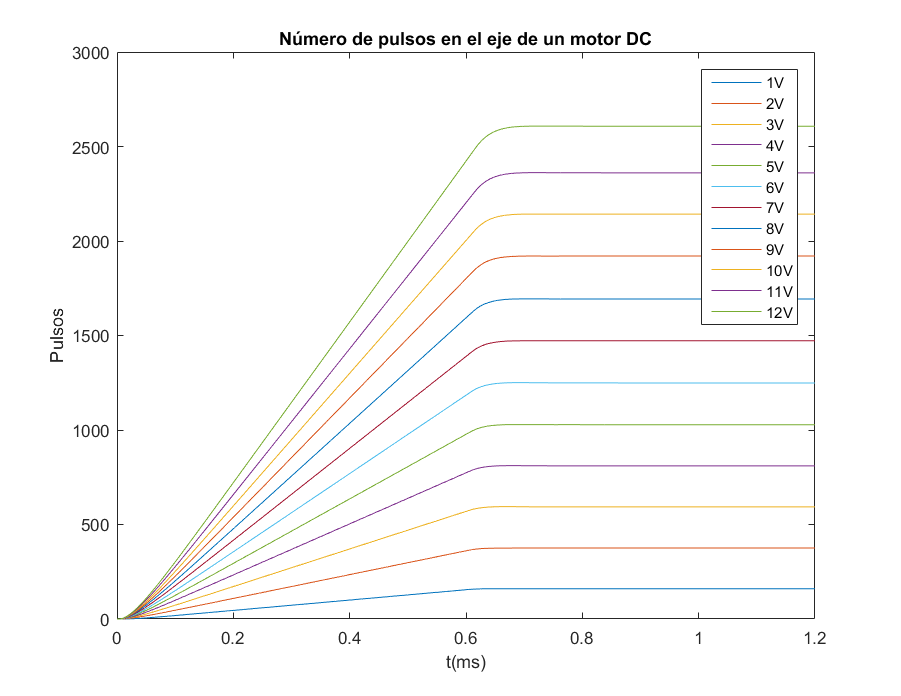
\includegraphics[width=8cm]{n_pulsos}
		\caption{Datos obtenidos del motor DC.\label{datos}}
	\end{center}
\end{figure}



\begin{thebibliography}{99}
\bibitem{git} \href{https://github.com/jjalberca/reallabo2018}{Repositorio del proyecto alojado en GitHub}
\bibitem{modelado} Félix Monasterio-Huelin y Álvaro Gutiérrez: \href{http://robolabo.etsit.upm.es/asignaturas/seco/apuntes/modelado.pdf}{Modelado de un motor DC}
\end{thebibliography}


\end{document}
